\documentclass{beamer}

\usepackage[russian]{babel}
\usepackage[utf8]{inputenc}
\usepackage{cmap}
\usepackage{graphicx}
\usepackage{xspace}
\usepackage{psfrag}

\newcommand{\MARK}[1]{{\bf {\it #1}}}
\newcommand{\CODE}[1]{{\ttfamily #1}}

\setbeamertemplate{footline}[frame number]
\usecolortheme{seahorse}
\beamertemplateshadingbackground{white}{blue!3}

\begin{document}
\sloppy

\begin{frame}
\begin{center}
Жарков Денис\\
\vspace{1cm}
{\Large Исследование методов автоматизированной обработки материалов \\ 
свободной энциклопедии Wikipedia\\
и алгоритма оценки близости предложений}
\end{center}
\begin{tabbing}
\hspace{6.5cm} \= Научный руководитель\\
\> кандидат.~тех.~наук\\
\> Пожидаев Михаил Сергеевич\\
\end{tabbing}
\end{frame}

\begin{frame}
\frametitle{Значимость Wikipedia как базы знаний}

\url{http://wikipedia.org}

\begin{itemize}
\item{
Строгая формализованность способа хранения статей;
}
\item{
в~подавляющем большинстве случаев справедливо
правило ``\textit{одна статья --- одно понятие}'';
}
\item{
множество ссылок указывают на~взаимосвязи между понятиями;
}
\item{
высокая достоверность данных, достигнутая засчет строгого контроля редакций.
}
\end{itemize}
\end{frame}

\begin{frame}
\frametitle{Выделенные задачи}
\begin{enumerate}
\item {
Анализ формата базы данных Wikipedia и реализация удобного программного интерфейса 
для~доступа к~данным.
}
\item {
Изучение существующих программных решений для работы с естественными языками (\textit{CoreNLP},\textit{WordNet}).
}
\item {
Исследование и анализ алгоритмов определения семантической близости предложений.
}
\item{
Реализация одного из алгоритмов определения семантической близости предложений и
анализ полученных результатов.
}
\end{enumerate}
\end{frame}

\begin{frame}
\frametitle{Формат архива Wikipedia}
База данных Wikipedia представляет собой XML-файл, в~котором
все статьи сохранены в~виде тэгов ``page'' верхнего уровня. 
Каждый из~них содержит следующие вложенные теги:

\begin{itemize}
\item{{\it title} --- заголовок, уникальный в~рамках всего множества статей;}
\item{{\it id} --- уникальный идентификатор статьи (положительное целое число);}
\item{{\it revision} --- описание последнего изменения статьи (дата, автор);}
\item{{\it text} --- последняя версия текста статьи.}
\end{itemize}
\end{frame}

\begin{frame}
\frametitle{Архитектура XML-парсера архива Wikipedia}
\begin{figure}
\begin{center}
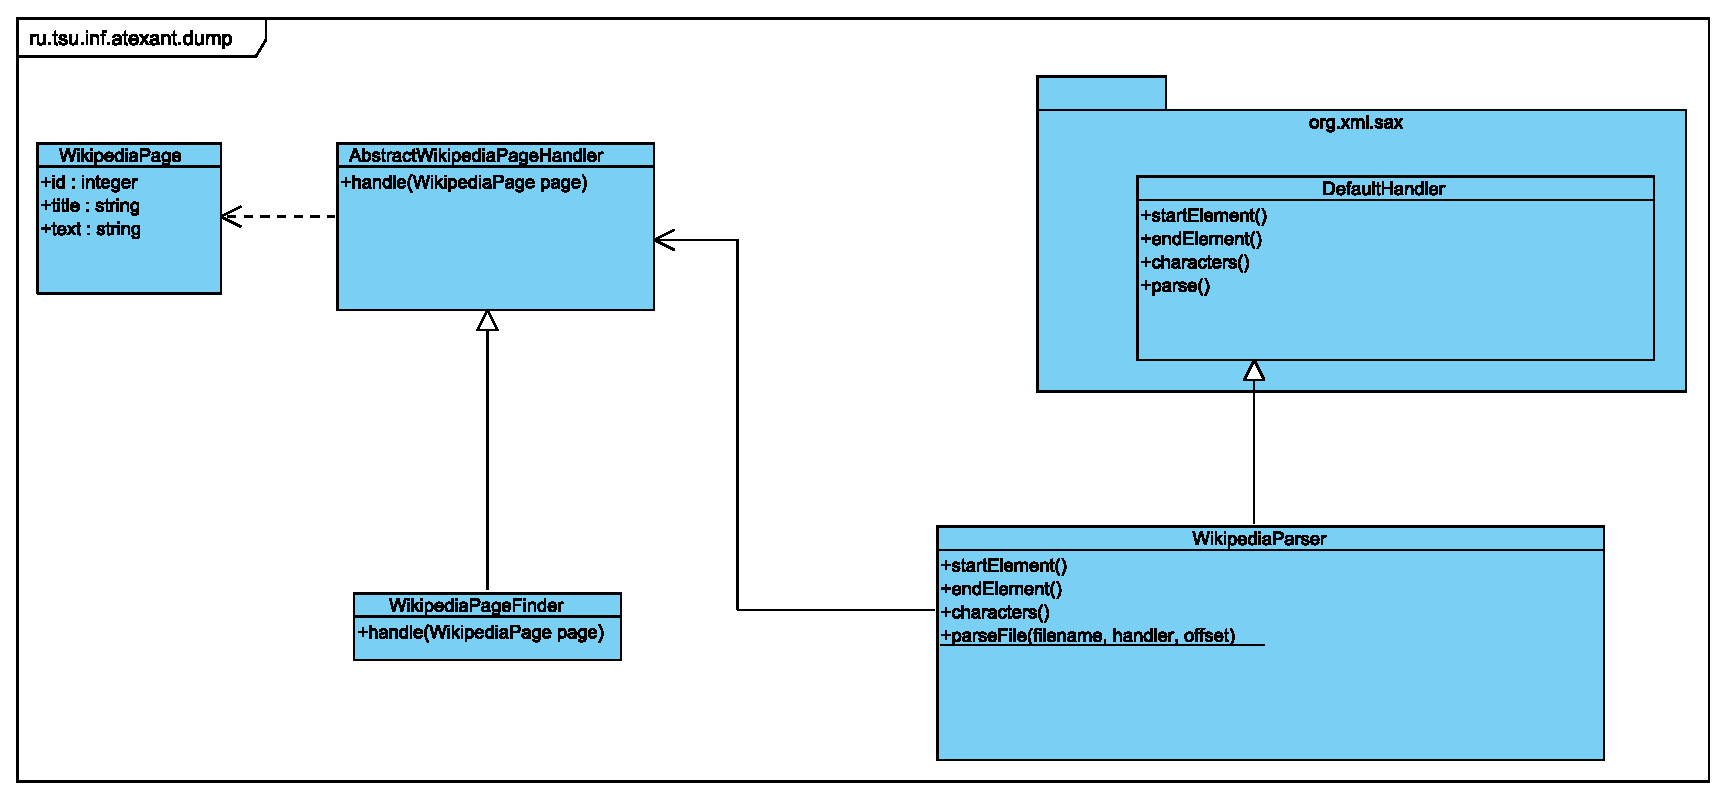
\includegraphics[scale=0.39]{../eps/ru.tsu.inf.atexant.dump.eps}
\end{center}
\end{figure}
\end{frame}

\begin{frame}
\frametitle{Разметка Mediawiki}

Помимо основного содержания,
текст статей Wikipedia включает в~себя элементы специальной разметки, 
которые позволяют:

\begin{enumerate}

\item{Управлять внешним видом блоков текста (размер/тип шрифта, цвет, отступ и~т.~п.).}
\item{Определять структуру документа (таблицы, вложенные списки, оглавления).}
\item{Выделять некоторые части текста как ссылки на~другие статьи.}

\end{enumerate}

{\it JWPL (Java Wikipedia Library) } - 
предоставляет программный доступ к~отдельным элементам разметки,
а также к тексту статьи, очищенному от разметки.
\end{frame}

\begin{frame}
\frametitle{Хранение в базе данных}

Для~более удобного доступа к~статьям,
было принято решение сохранять информацию о~каждой из~них 
в~реляционной СУБД \textit{MySQL} в~таблице со~следующими столбцами:

\begin{itemize}
\item{числовой идентификатор;}
\item {заголовок;}
\item {в~случае перенаправления, заголовок и идентификатор базовой статьи;}
\item {
сдвиг в~байтах от~начала архива-исходника, 
где расположена страница.
}
\end{itemize}

Предполагается переход к~более производительным БД, 
таким как Lucene или MongoDB. 

\end{frame}

\begin{frame}
\frametitle{CoreNLP}
Пакет Stanford CoreNLP --- это один из~самых развитых инструментов для~работы с~естественными языками, 
первая версия которого датируется 1~ноября~2010~г.
Он является набором классов на языке Java, предоставляющих интерфейсы для~решения многочисленных проблем NLP. 

В~настоящей работе использовались две подсистемы CoreNLP:

\begin{enumerate}

\item {{\it POS-tagger}, предназначенный для~определения частей речи слов и их~лемматизации.}
\item {{\it Parser}, предоставляющий возможность строить дерево зависимостей членов предложений.}

\end{enumerate}

\end{frame}

\begin{frame}
\frametitle{CoreNLP и представление деревьев зависимостей}
Предложение: {\it ``If I had a gun I'd shoot a hole into the sun''}

Его список зависимостей имеет вид:
%%я постараюсь успеть нарисовать дерево чуть позже

\begin{center}

mark(had-3, If-1)\\
nsubj(had-3, I-2)\\
root(ROOT-0, had-3)\\
det(gun-5, a-4)\\
dobj(had-3, gun-5)\\
nsubj(shoot-8, I-6)\\
aux(shoot-8, 'd-7)\\
rcmod(gun-5, shoot-8)\\
det(hole-10, a-9)\\
dobj(shoot-8, hole-10)\\
prep(shoot-8, into-11)\\
det(sun-13, the-12)\\
pobj(into-11, sun-13)\\

\end{center}

\end{frame}

\begin{frame}
\frametitle{Задача определения семантической близости предложения}

Введём меру близости, как функцию от~двух аргументов-предложений, отвечающую следующим требованиям:

\begin{enumerate}

\item {
Её~значения находятся в~интервале $[0,1]$.
}

\item {
Если взять значения этой меры для~двух различных пар предложений, 
то большее значение должно соответствовать той паре, которая по~мнению большей группы опрошенных людей считается более близкой по~смыслу.
}

\end{enumerate}
\end{frame}

\begin{frame}
\frametitle{Алгоритмы первого типа определения семантической близости предложений}

Алгоритмы первого типа --- это алгоритмы, которые рассматривают предложения и отдельные слова только как символьные строки, 
определяя меру близости на~основе разнообразных статистических методов, 
руководствуясь при~этом только сходством в~написании слов.

\end{frame}

\begin{frame}
\frametitle{Алгоритмы второго типа определения семантической близости предложений}

\begin{enumerate}
\item{
Для~исходных предложений строится полный взвешенный двудольный граф, 
вершинами которого являются отдельные слова каждого из~предложений, 
а вес каждого из~ребер равен значению меры близости слов $Sim_{words}(w_1, w_2)$,
соответствующих вершинам на~концах ребра. 
}
\item{
$Sim_{words}(w_1, w_2)$ --- величина, значения которой также принадлежат интервалу $[0,1]$.
Показывает, насколько слова $w_1,w_2$ семантически близки.
}
\item{
Решается задача о назначении, в которой
нужно каждому слову первого предложения поставить в соответствие одно слово из второго,
так, чтобы максимизировать суммарную близость всех пар.
}
\end{enumerate}

\end{frame}

\begin{frame}
\frametitle{Алгоритмы третьего типа определения семантической близости предложений}

\begin{enumerate}

\item {
Строятся деревья зависимостей оцениваемых предложений.
}

\item {
Для каждой зависимости $d$ определяется ее  вес $weight(d)$, равный величине,  
зависимой от~расстояния до~корня дерева.
}

\item{
$d2dSim(d_1,d_2) = \lambda_1 \cdot Sim_{words}(h(d_1),h(d_2)) + \lambda_2 \cdot Sim_{words}(m(d_1),m(d_2)), $
где $d_1, d_2$ --- пара сравниваемых зависимостей,\\
$h(d_i), m(d_i)$ --- управляющее и подчиненное слова зависимости $d_i$,\\
$Sim_{words}(w_1,w_2)$ --- мера близости слов, найденная с использованием Wordnet,\\
а $\lambda_1 + \lambda_2 = 1$.
}

\item{
$paraphrase(S_1, S_2) = sim(S_1,S_2)/diss(S_1, S_2)$, 
где $sim(S_1, S_2)$ --- это вес максимального паросочетания,
а $diss(S_1, S_2)$ --- сумма весов ``значимости'' для~беспарных зависимостей.
}
\end{enumerate}

\end{frame}

\begin{frame}
\frametitle{Задача определения семантической близости предложения. Алгоритмы комплексного анализа}

Вариант декомпозиции:
\begin{itemize}
\item{
Семантическая близость предложений;
}
\item{
Cинтаксическая близость предложений;
}
\end{itemize}

\end{frame}

\begin{frame}
\frametitle{Семантическая близость предложений}

$sim_{sem}(S_1 , S_2) = \beta_1 \cdot sim_{nsets}(v_1, v_2) + \beta_2 \cdot sim_{nsets}(\eta_1, \eta_2), $\\
где
$\beta_1 + \beta_2 = 1$.\\
\vspace{0.5cm}
Для сравнения множеств вершин $A_1,A_2$ вводится векторное пространство размерности $|A_1 \cup A_2|$.

$A_1,A_2$ ставятся в соответствие вектора $\vec{a_1},\vec{a_2}, $ 
а $n_l$ --- $l$-ое слово из множества $A_1 \cup A_2$ --- соответствует l-ому базисному вектору.
$$a_{1l} = \max(sim_{nodes}(n_l, A_{1j})) \text{ для } j=\overline{1,|A_1|},$$
$$a_{2l} = \max(sim_{nodes}(n_l, A_{2j})) \text{ для } j=\overline{1,|A_2|},$$

$$ sim_{nsets}(A_1,A_2) = \cos\left(\vec{a_1},\vec{a_2}\right). $$

\end{frame}

\begin{frame}
\frametitle{Семантическая близость предложений}

$$ sim_{nodes}(N_1, N_2) = \gamma_1 \cdot sim_{words}(w_1,w_2) + \gamma_2 \cdot sim_{sets}(D_{w1}, D_{w2}), $$
где $w_1, w_2$ --- главные слова вершин $N_1, N_2$, а $D_{w1}, D_{w2}$ --- множества слов-потомков этих вершин,
причем $\gamma_1+\gamma_2=1$.

$$sim_{sets}(D_1, D_2) = \frac{sim_{D}(D_1,D_2) + sim_{D}(D_2, D_1)}{2}, $$
а 
$$sim_{D}(D_1, D_2) = \frac{ \sum \limits_{i=1}^{|D_1|} \max_{j=1,|D_2|} sim_{words}(D_{1i}, D_{2j}) } { |D1| }$$

\end{frame}

\begin{frame}
\frametitle{Синтаксическая близость предложений}
Список ребер вида:\\

\textit{<часть речи упр. слова, часть речи под. слова, тип связи>}.

$S_{syn_1}$ и $S_{syn_2}$ --- множества ребер 
модифицированных деревьев зависимостей двух предложений.\\
\vspace{0.2cm}
Итоговая формула синтаксической близости имеет вид: 
$$sim_{syn}(S_1, S_2) = 2 \cdot |S_{syn_1} \cup S_{syn_2}| / (|S_{syn_1}| + |S_{syn_2}|),$$ 
\vspace{0.1cm}
Как результат оценивания суммарной меры близости предложений, 
дается следующая формула:
$$sim(S_1, S_2) = \alpha_1 \cdot sim_{sem}(S_1, S_2) + \alpha_2 \cdot sim_{syn}(S_1, S_2),$$
 при $\alpha_1+\alpha_2=1$,

\end{frame}

\begin{frame}
\frametitle{Реализация алгоритма комплексного анализа}

Среднее значение отклонения: $0.150915$.\
\vspace{0.1cm}
Наибольшее значение погрешности ($0.361794$) было получено для пары предложений:
\begin{itemize}
\item {
	A boy is a child who will grow up to be a man.
}
\item {
	A rooster is an adult male chicken.
}
\end{itemize}
где значение оценки, данной людьми, составляет $0.1075$, а результат алгоритма --- $0.469294$.

\end{frame}

\begin{frame}
\frametitle{Поиск предложений в Wikipedia}

\vspace{0.2cm}
Статья Wikipedia: ``Alchemy''.\\
Исходное предложение:\\
\textit{"The best known goals of the alchemists were the transmutation of common metals into Gold or Silver, and the creation of a "panacea," a remedy that supposedly would cure all diseases and prolong life indefinitely; and the discovery of a universal solvent."}

Измененное:

\textit{"The most famous targets of the alchemist's is the transformation of common metals into gold, and making of a magic remedy named panacea".}

В~результате запуска алгоритма в~качестве наиболее похожего 
было выбрано исходное предложение со~значением меры близости $0.334027866$.
\end{frame}

\begin{frame}
\frametitle{Заключение}

\begin{enumerate}
\item {
Реализован программный пакет, позволяющий получить доступ к~тексту
и отдельным элементам разметки отдельных страниц.
}
\item {
Модуль для~сохранения статей из~архива Wikipedia
в~СУБД~MySQL.
}
\item {
Проведены исследования и условная классификация существующих 
алгоритмов определения меры семантической близости предложений. 
Проанализированы и показаны их достоинства и недостатки.
}
\item {
Реализован один из~рассмотренных алгоритмов с~запуском для~набора 
пар предложений, близость которых была оценена людьми. 
}
\item {
Изучены программные продукты для работы
с~естественными языками, такие как CoreNLP и WordNet.
} 
\item {
Выдвинуты предложения по улучшению реализованного алгоритма.
}
\end{enumerate}
\end{frame}

\begin{frame}
{\Large Спасибо за внимание!}
\end{frame}

\end{document}
